\chapter{CRUD WITH SPRING AND THYMELEAF}

Spring adalah sebuah \textit{framework} yang memudahkan kita membangun sebuah aplikasi baik itu aplikasi berbasis desktop, web, ataupun \textit{mobile}.

Cara paling mudah untuk memulai menggunakan framework Spring adalah dengan mengunjungi situs \url{https://spring.io}, dan saat akan memulai sebuah \textit{project} kita dapat menggunakan rangka \textit{project} yang disediakan oleh Spring di halaman \url{http://start.spring.io}, tampilan halaman web-nya akan terlihat seperti pada gambar \ref{fig:start-spring} :

\begin{figure}[H]
	\centering
	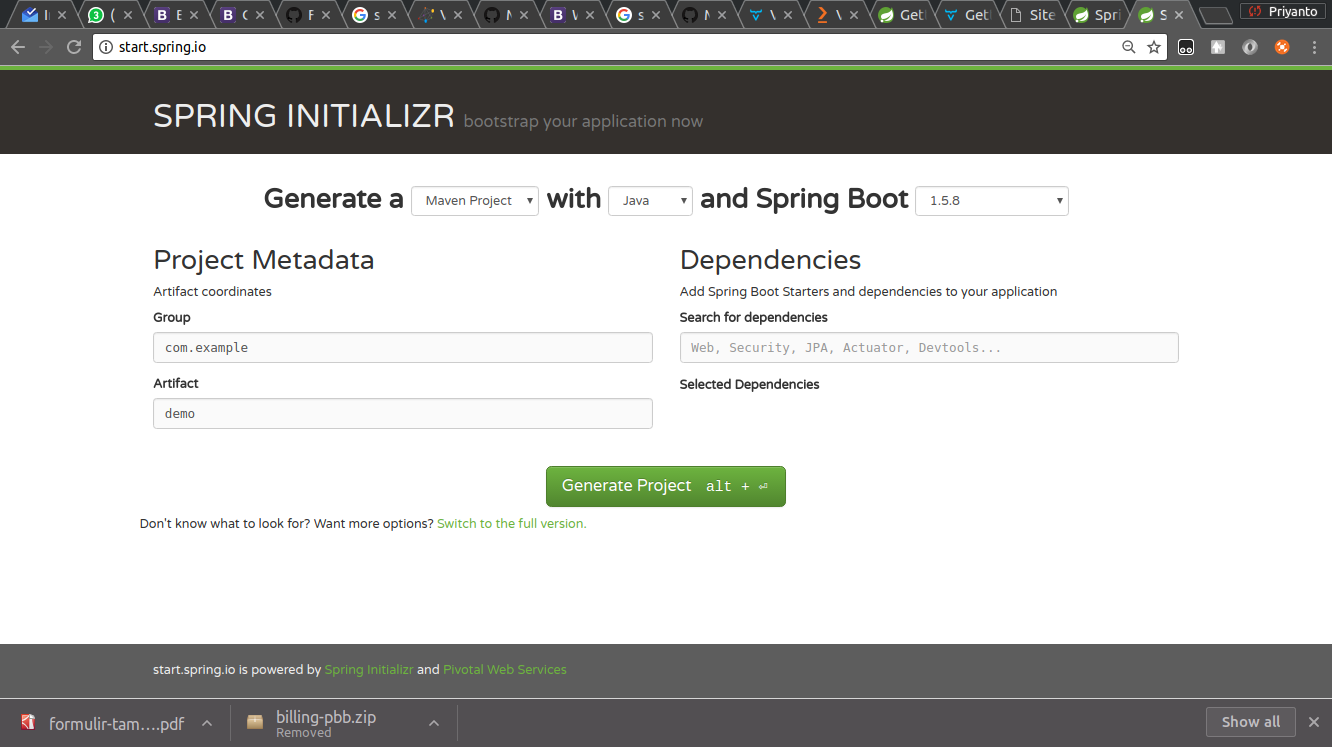
\includegraphics[width=1\textwidth]{./resources/001-tampilan-start-spring}
	\caption{Tampilan start.spring.io}
	\label{fig:start-spring}
\end{figure}

Yang perlu diisikan dari form yang ada pada website \url{start.spring.io} adalah sebagai berikut :

\begin{itemize}
	\item \textbf{Group} yang diisikan dengan nama atau identitas organisasi, instansi, atau tim yang mengembangkan aplikasi. Pengisian disini biasanya akan dijadikan nama paket dalam kandar (\textit{folder}) kode sumber (\textit{source code}).
	\item \textbf{Artifact} yang diisikan dengan nama aplikasinya. Sebaiknya jangan menggunakan titik disini, isikan hanya dengan huruf dan angka.
	\item \textbf{Dependencies} yang diisikan dengan pustaka-pustaka (\textit{library}) yang nantinya akan digunakan dalam \textit{project}.
\end{itemize}

Setelah itu klik tombol \texttt{Generate Project} atau tekan tombol \texttt{Ctrl + Enter} di tombol \textit{keyboard}. Nanti kita akan mendapat sebuah \textit{file} terkompres dengan ekstensi \texttt{zip}, ekstraklah \textit{file} ini untuk selanjutnya kita buka dalam IDE Netbeans.

\section{Uji Coba Pertama}

Untuk pertama kalinya, kita akan mencoba bagaimana cara kerja Spring Framework dalam membangun sebuah aplikasi web dengan konsep MVC (\textit{Model-View-Controller}). Berikut langkahnya :

\begin{enumerate}
	\item Buat kerangka \textit{project} dari laman \url{start.spring.io} dengan isian pustakanya adalah \textbf{Web} dan \textbf{Thymeleaf} seperti gambar \ref{fig:create-spring} :
	
	\begin{figure}[H]
		\centering
		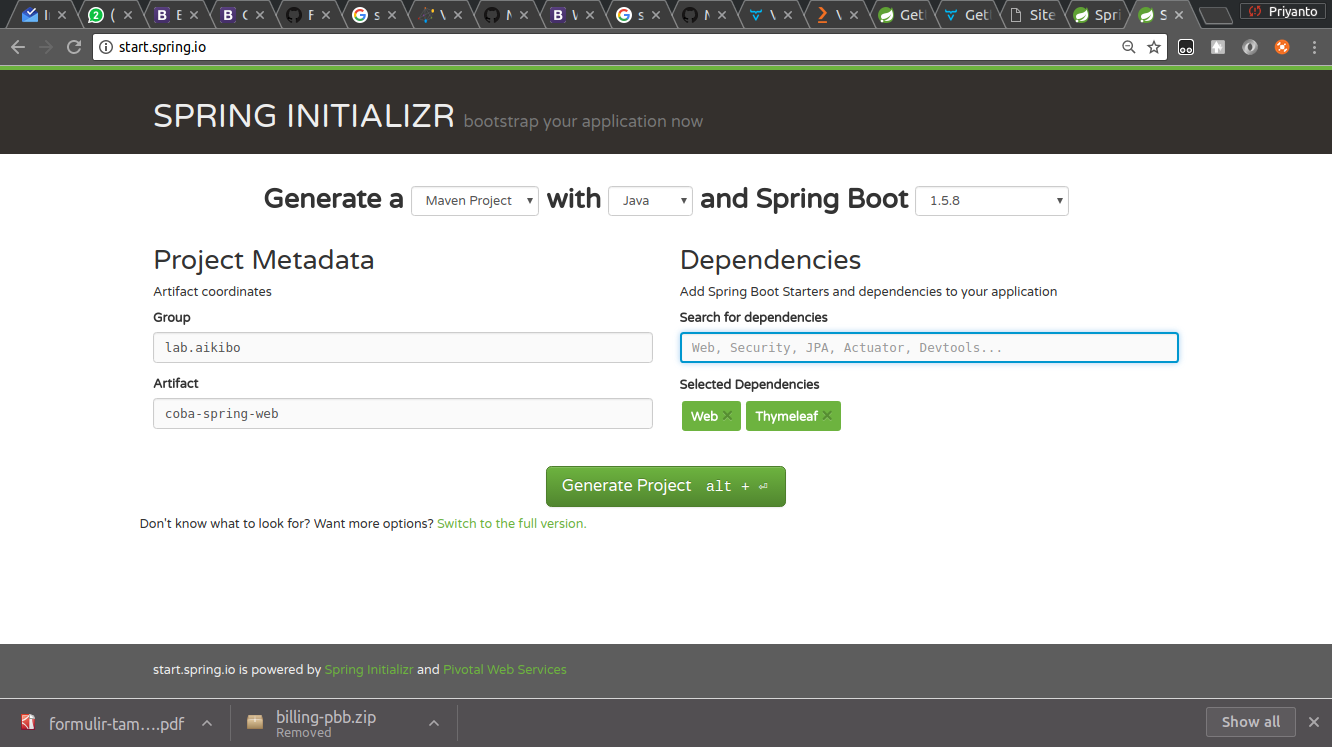
\includegraphics[width=1\textwidth]{./resources/002-create-spring}
		\caption{Membuat Rangka \textit{Project}}
		\label{fig:create-spring}
	\end{figure}
	
	\item Setelah \textit{file} diekstrak, bukalah dengan Netbeans sehingga terlihat struktur \textit{folder} seperti pada gambar \ref{fig:struktur-project} :
	
	\begin{figure}[H]
		\centering
		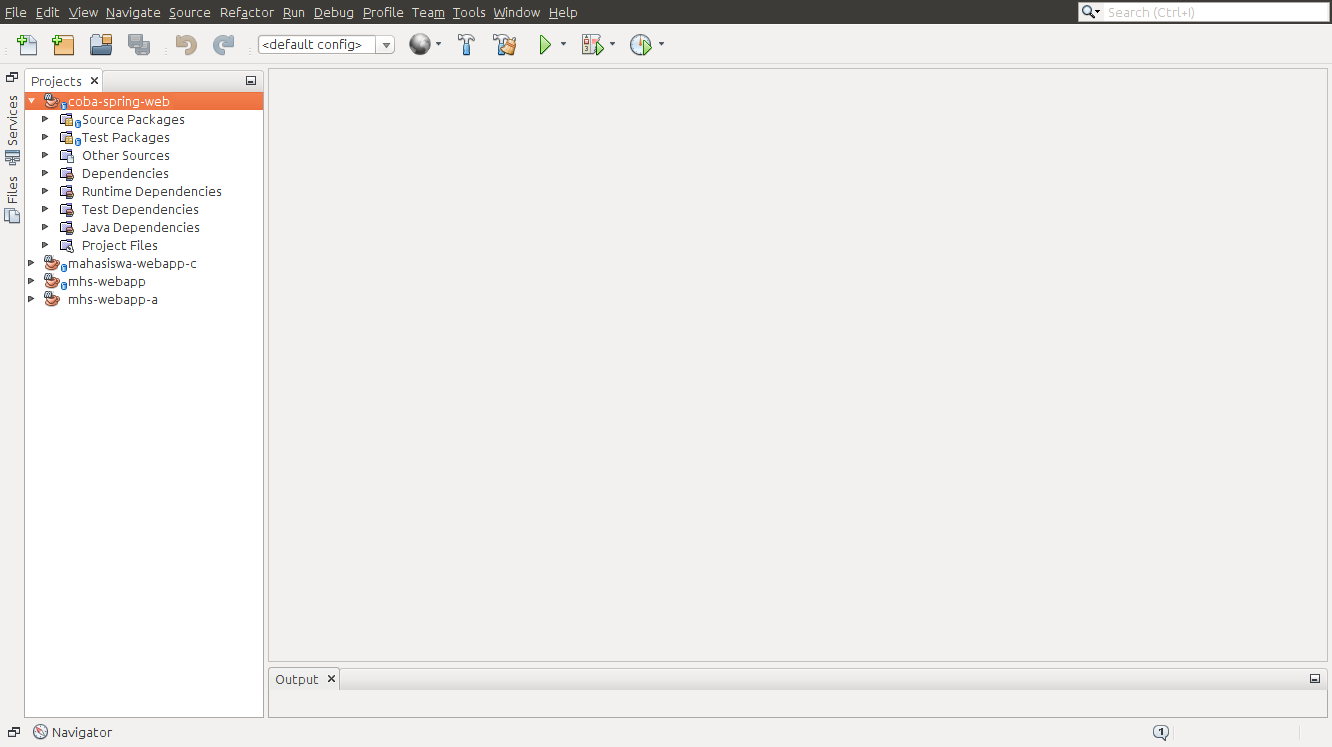
\includegraphics[width=1\textwidth]{./resources/003-struktur-di-netbeans}
		\caption{Struktur Direktori \textit{Project}}
		\label{fig:struktur-project}
	\end{figure}
	
	\item Buatlah sebuah \textit{file} \texttt{html} sebagai bagian dari \textit{View} dalam konsep MVC di bagian \texttt{Other Sources}, di bagian \texttt{templates} berikan nama bebas, misal kita berikan nama \texttt{home.html} dengan isian sebagai berikut :
	
	\begin{lstlisting}
<html>
    <head>
        <title>Aplikasiku</title>
    </head>
    <body>
        <h1>Selamat Datang</h1>
    </body>
</html>
	\end{lstlisting}
	
	\textit{File} \texttt{home.html} di Netbeans akan disimpan seperti gambar \ref{fig:posisi-home-html} :
	
	\begin{figure}[H]
		\centering
		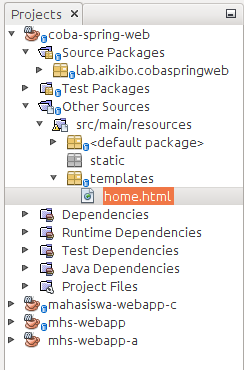
\includegraphics[width=0.5\textwidth]{./resources/004-posisi-home-html}
		\caption{Posisi \textit{File} \texttt{home.html}}
		\label{fig:posisi-home-html}
	\end{figure}
	
	\item Berikutnya kita buatkan sebuah \textit{controller} yang menghubungkan antara aplikasi \textit{backend} dengan \textit{frontend}, biasanya untuk \textit{controller} ini dibuatkan dalam sebuah paket tersendiri dalam \texttt{Source Packages} dengan nama \texttt{controller}. Buatlah sebuah \textit{file controller} disana, misalkan kita beri nama \texttt{AppController} seperti terlihat pada gambar \ref{fig:posisi-appcontroller} :
	
	\begin{figure}[H]
		\centering
		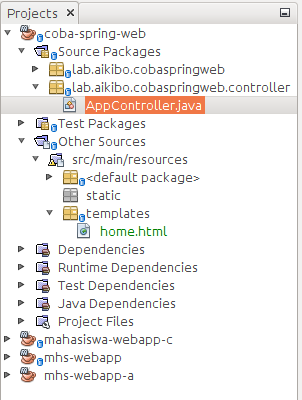
\includegraphics[width=0.5\textwidth]{./resources/005-posisi-appcontroller}
		\caption{Posisi \textit{File} \texttt{AppController.java}}
		\label{fig:posisi-appcontroller}
	\end{figure}
	
	Isi kode dari \textit{file} \texttt{AppController.java} adalah sebagai berikut :
	
	\begin{lstlisting}
package lab.aikibo.cobaspringweb.controller;

import org.springframework.stereotype.Controller;
import org.springframework.web.bind.annotation.RequestMapping;

/**
 *
 * @author tamami <tamami.oka@gmail.com>
 */
@Controller
public class AppController {
    
    @RequestMapping("/home")
    public void index() {}
    
}
	\end{lstlisting}

	Perhatikan bahwa parameter dari \texttt{@RequestMapping} harus sama dengan nama \textit{file} \texttt{html} yang kita buat sebelumnya.

	\item Jalankan aplikasinya dengan tombol \texttt{F6} di \textit{keyboard}, kemudian pilih saja \texttt{Main Class} yang sudah disediakan, atau jalankan \textit{main file} yang dibentuk oleh Spring, carilah sebuah kelas yang didalamnya ada anotasi \texttt{@SpringBootApplication} dan memiliki sebuah \textit{method} \texttt{main} seperti gambar \ref{fig:main-class} :
	
	\begin{figure}[H]
		\centering
		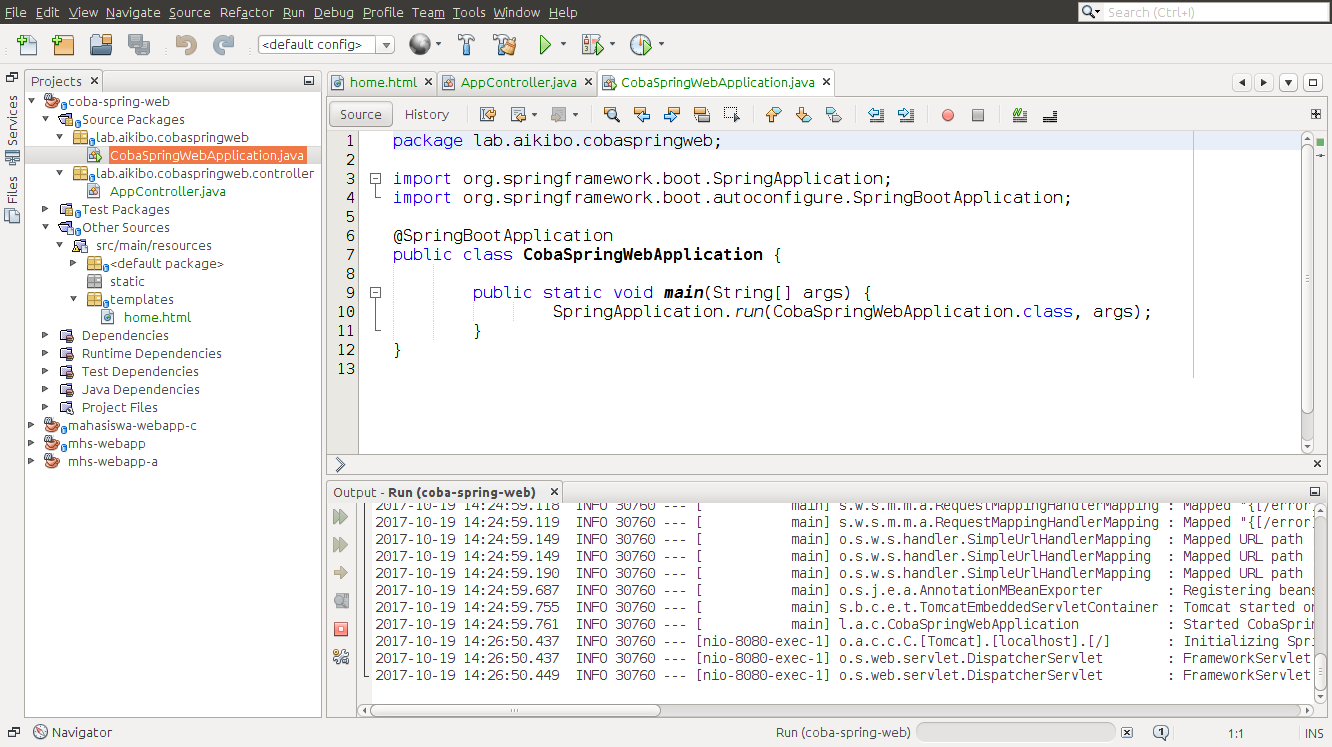
\includegraphics[width=1\textwidth]{./resources/006-main-class}
		\caption{\textit{Main Class}}
		\label{fig:main-class}
	\end{figure}
	
	Klik kanan lalu pilih \texttt{Run File} atau tekan tombol \texttt{Shift + F6} di \textit{keyboard}.
	
	\item Bukalah \textit{browser}, lalu akses ke alamat \texttt{localhost:8080}, sehingga seharusnya akan muncul tampilan seperti gambar \ref{fig:localhost-1} :
	
	\begin{figure}[H]
		\centering
		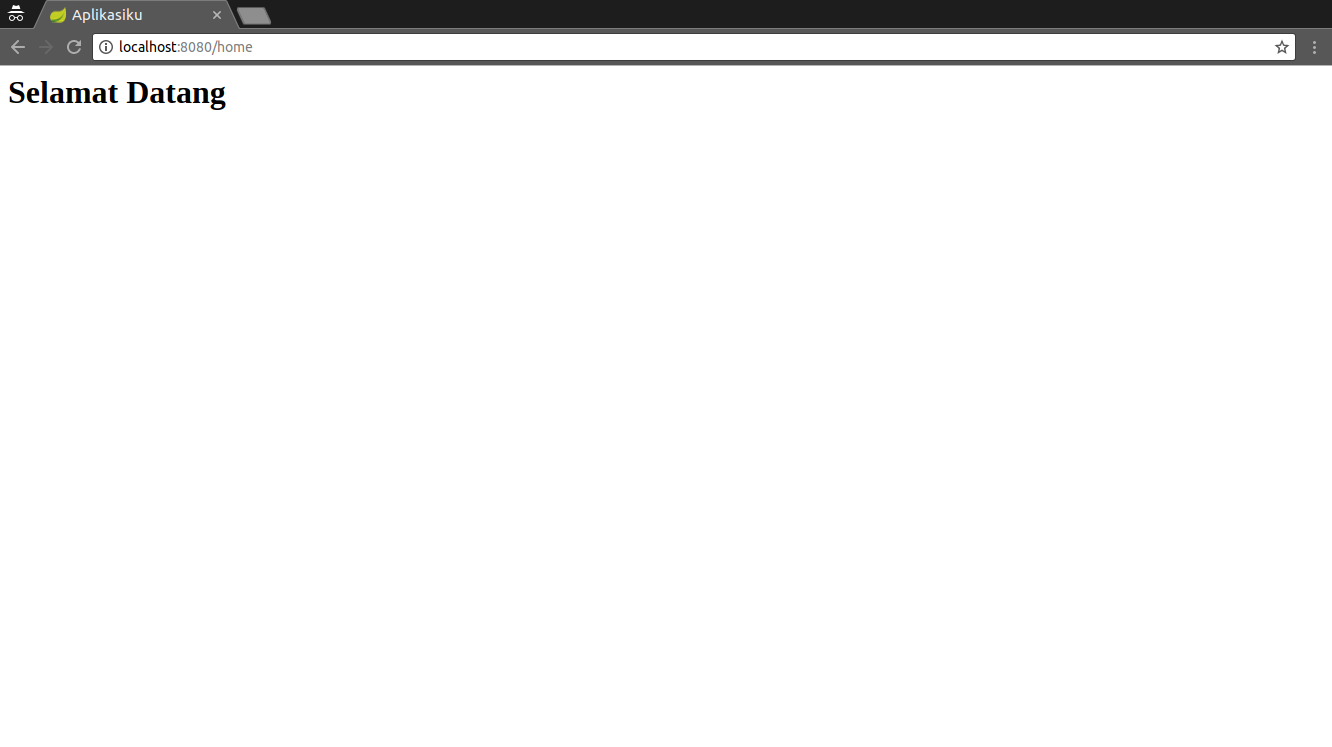
\includegraphics[width=1\textwidth]{./resources/007-localhost-1}
		\caption{Halaman Yang tampil Pertama Kali}
		\label{fig:localhost-1}		
	\end{figure}
\end{enumerate}

Sampai sini, kita telah melihat bahwa konsep MVC diimplementasikan dalam Spring Web secara utuh dan terlihat strukturnya, selanjutnya kita akan coba menampilkan isi dari basis data ke jendela web aplikasi kita.

\section{Tampilkan Data}

Sebelum kita tampilkan datanya, datanya harus disiapkan terlebih dahulu. Struktur data yang perlu dibentuk adalah sebagai berikut :

\begin{tabular}{| c | c | c |}
	\hline
	Kolom & Tipe & Keterangan \\
	\hline \hline
	nim & varchar(7) & not null primary key \\
	\hline
	nama & varchar(30) & \\
	\hline
	jurusan & varchar(50) & \\
	\hline
\end{tabular}

Berikan data \textit{sample} untuk kita lakukan uji coba awal, yaitu menampilkan data di halaman aplikasi \textit{web} yang kita bangun.

Data yang disiapkan untuk modul ini kebetulan menggunakan basis data PostgreSQL, yang nantinya akan ada perbedaan konfigurasi bila menggunakan basis data yang lain, namun jangan khawatir karena informasi untuk konfigurasi basis data yang lain seperti MySQL cukup mudah ditemukan di internet.

Untuk mempermudah langkah kita membangun sebuah aplikasi ini, kita kunjungi lagi alamat \url{start.spring.io} dengan beberapa pustaka seperti pada gambar \ref{fig:init-project-crud} :

\begin{figure}[H]
	\centering
	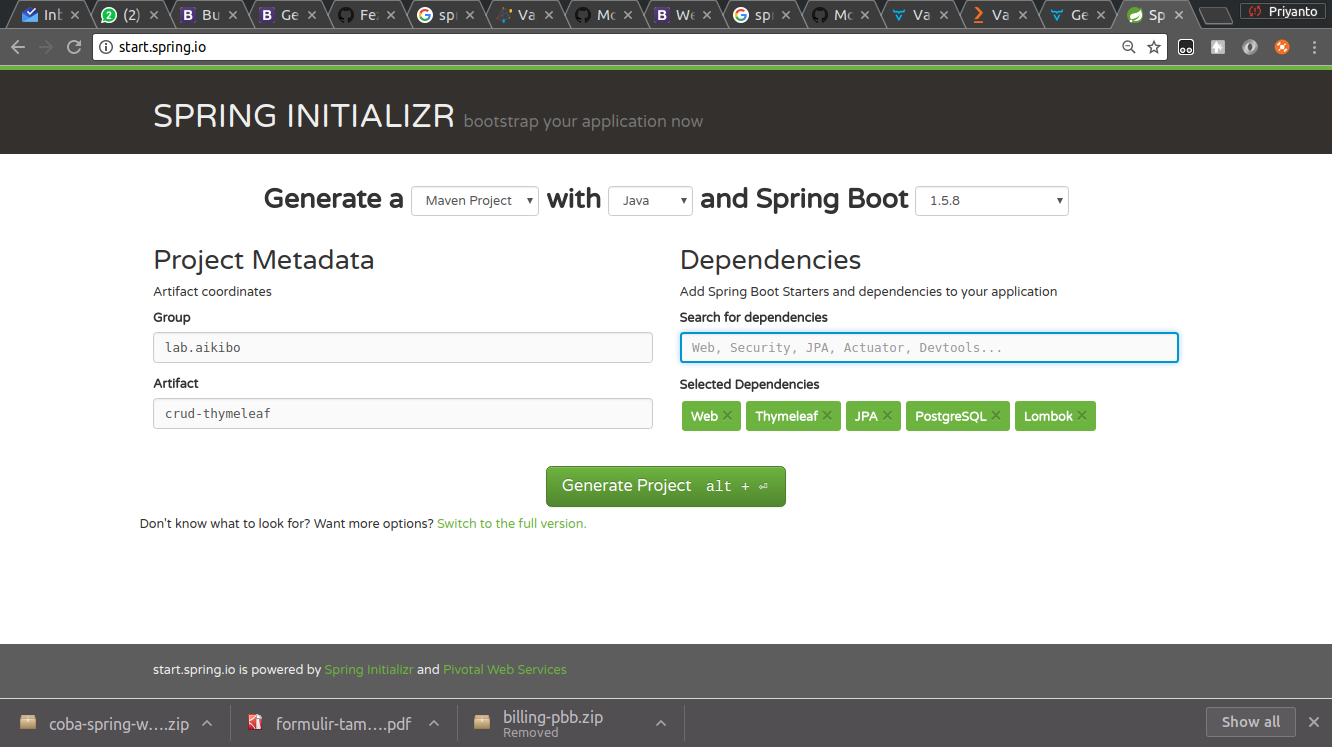
\includegraphics[width=1\textwidth]{./resources/008-init-project-crud}
	\caption{\textit{Generate Project} Untuk CRUD}
	\label{fig:init-project-crud}
\end{figure}

Seperti sebelumnya, \textit{file} \texttt{zip} yang telah diunduh kita ekstrak dan buka dengan IDE Netbeans / Sublime / IDE / \textit{editor} lainnya.

Berikut langkah bagaimana kita dapat menampilkan data tabel dari basis data yang kita buat sebelumnya ke halaman aplikasi web yang kita buat :

\begin{enumerate}
	\item Pertama kita buat konfigurasi koneksi ke basis data agar Spring Data JPA dapat melakukan akses data secara penuh ke sistem basis data yang kita gunakan. Konfigurasi ini ada pada \textit{file} \texttt{application.properties} di dalam bagian \texttt{Other Sources} pada \texttt{<default package>}. Gambar \ref{fig:lokasi-application-properties} menunjukkan lokasi \textit{file} \texttt{application.properties}. 
	
	\begin{figure}[H]
		\centering
		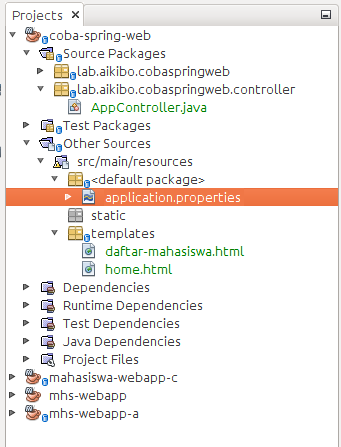
\includegraphics[width=0.5\textwidth]{./resources/010-lokasi-application-properties}
		\caption{Lokasi \textit{File} \texttt{application.properties}}
		\label{rfig:lokasi-application-properties}
	\end{figure}
	
	Untuk yang menggunakan basis data PostgreSQL, isi konfigurasinya adalah sebagai berikut :
	
	\begin{lstlisting}
spring.datasource.url = jdbc:postgresql://localhost:5432/phb
spring.datasource.username = dev
spring.datasource.password = rahasia
spring.datasource.driver-class-name = org.postgresql.Driver

spring.jpa.database-platform = org.hibernate.dialect.PostgreSQL9Dialect
	\end{lstlisting}
	
	Format untuk \texttt{url} sendiri yang biasanya berubah adalah bagian \texttt{phb}, karena ini adalah nama \textit{database} yang digunakan, bila menggunakan nama yang lain, silahkan diubah. Hal lain yang perlu disesuaikan tentu saja adalah bagian \texttt{username} dan \texttt{password}.
	
	Isi konfigurasi bila kita menggunakan MySQL akan menjadi seperti berikut :
	
	\begin{lstlisting}
spring.datasource.url = jdbc:mysql://localhost:3306/mahasiswa
spring.datasource.username = dev
spring.datasource.password = rahasia
spring.datasource.driver-class-name = com.mysql.jdbc.Driver

spring.jpa.database-platform = org.hibernate.dialect.MySQLDialect
	\end{lstlisting}
	
	\item Selanjutnya kita buat dahulu \textit{file} \texttt{html} sebagai \textit{user interface} yang akan menampilkan isi dari tabel \texttt{mahasiswa}, \textit{file} ini harus ditempatkan dalam pada bagian \texttt{Other Sources} di dalam \textit{folder} \texttt{templates} seperti terlihat pada gambar \ref{fig:tempat-daftar-mahasiswa} berikut :
	
	\begin{figure}[H]
		\centering
		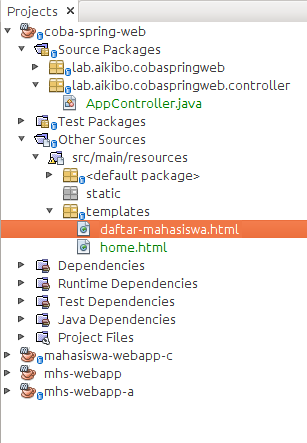
\includegraphics[width=0.5\textwidth]{./resources/009-tempat-daftar-mahasiswa}
		\caption{Lokasi \textit{File} \texttt{daftar-mahasiswa.html}}
		\label{fig:tempat-daftar-mahasiswa}
	\end{figure}
	
	Isi dari \textit{file} \texttt{daftar-mahasiswa.html} ini adalah sebagai berikut :
	
	\begin{lstlisting}
<html xmlns:th="http://www.thymeleaf.org">
    <head>
        <title>Daftar Mahasiswa</title>
        <meta charset="UTF-8" />
        <meta name="viewport" 
              content="width=device-width, initial-scale=1.0"/>
    </head>
    <body>
        <h1>Daftar Mahasiswa</h1>
        
        <table border="1">
            <thead>
                <tr>
                    <th>NIM</th>
                    <th>NAMA</th>
                    <th>JURUSAN</th>
                </tr>
            </thead>
            <tbody>
                <tr th:each="mhs : ${daftarMahasiswa}">
                    <td th:text="${mhs.nim}"></td>
                    <td th:text="${mhs.nama}"></td>
                    <td th:text="${mhs.jurusan}"></td>
                </tr>
            </tbody>
        </table>
    </body>
</html>
	\end{lstlisting}	
	
	Perhatikan pada baris ke-20, disana ada deklarasi variabel \texttt{mhs} yang nantinya akan diisikan oleh setiap nilai yang ada pada variabel \texttt{daftarMahasiswa}. Variabel \texttt{daftarMahasiswa} sendiri sebetulnya akan dikirimkan dari \textit{controller} di \textit{server}.
	
	Nilai dari masing-masing \texttt{daftarMahasiswa} itu sebetulnya adalah sebuah objek yang nantinya dititipkan ke variabel \texttt{mhs} yang kemudian pada baris ke-21 sampai ke-23 akan ditampilkan satu-satu berdasarkan nama propertinya, yaitu \texttt{nim}, \texttt{nama}, dan \texttt{jurusan}.
	
	\item Selanjutnya adalah membuat \textit{controller} agar \textit{file} \texttt{html} yang kita buat dapat tampil di \textit{browser}. Gunakan saja \textit{controller} yang sudah ada, yaitu \texttt{AppController} dengan tambahan \texttt{RequestMapping} baru sehingga kodenya menjadi terlihat seperti berikut ini :
	
	\begin{lstlisting}
package lab.aikibo.cobaspringweb.controller;

import lab.aikibo.cobaspringweb.repo.MahasiswaRepo;
import org.springframework.beans.factory.annotation.Autowired;
import org.springframework.stereotype.Controller;
import org.springframework.ui.Model;
import org.springframework.web.bind.annotation.RequestMapping;

/**
 *
 * @author tamami <tamami.oka@gmail.com>
 */
@Controller
public class AppController {
    
    @Autowired
    private MahasiswaRepo mhsRepo;
    
    @RequestMapping("/home")
    public void index() {}
    
    @RequestMapping("/daftar-mahasiswa") 
    public void getDaftarMahasiswa(Model model) {
        model.addAttribute("daftarMahasiswa", mhsRepo.findAll());
    }
    
}
	\end{lstlisting}
	
	Perhatikan bahwa di kelas \texttt{controller} ini, ada anotasi baru yang kita gunakan, yaitu \texttt{Autowired} dimana ini adalah \textit{feature} dari Spring untuk \textit{dependency injection} yang secara otomatis akan membuatkan kita instan dari \textit{interface} \texttt{MahasiswaRepo}.
	
	Perhatikan juga pada baris ke-22, dimana kita membentuk \textit{mapping} baru untuk \texttt{daftar-mahasiswa}, kemudian pada \textit{method} \texttt{getDaftarMahasiswa} pada baris ke-23 memiliki sebuah parameter \texttt{model} yang merupakan pengait data antara \textit{backend service} dengan \textit{frontend service}.
	
	Yang terakhir adalah pada baris ke-24 dimana pada \texttt{model} ditambahkan atribut \texttt{daftarMahasiswa} sebagaimana dibutuhkan sebelumnya pada \textit{file} \texttt{daftar-mahasiswa.html}, yang isinya diambilkan dari basis data dengan memanggil \textit{repository} kelas hasil turunan / pewarisan dari \texttt{JpaRepository}.
	
	\item Membuat \textit{file interface} \texttt{MahasiswaRepo} yang kita simpan pada \textit{package} tersendiri. Gambar \ref{fig:lokasi-repo-package} menunjukkan lokasi dari \textit{package} \texttt{repo} berada. 
	
	\begin{figure}[H]
		\centering
		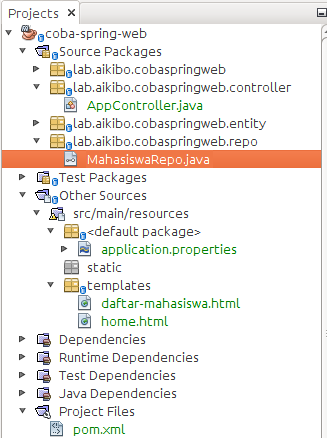
\includegraphics[width=0.5\textwidth]{./resources/011-lokasi-mhs-repo}
		\caption{Lokasi \textit{Packgae} Repo}
		\ref{fig:lokasi-repo-package}
	\end{figure}
	
	\item Kemudian membuat sebuah \textit{interface} didalamnya untuk melakukan operasi \textit{database}. Disini kita beri nama \texttt{MahasiswaRepo.java} dengan isi kodenya adalah sebagai berikut :
	
	\begin{lstlisting}
package lab.aikibo.cobaspringweb.repo;

import lab.aikibo.cobaspringweb.entity.Mahasiswa;
import org.springframework.data.jpa.repository.JpaRepository;
import org.springframework.stereotype.Repository;

/**
 *
 * @author tamami <tamami.oka@gmail.com>
 */
@Repository
public interface MahasiswaRepo extends JpaRepository<Mahasiswa, String> {
    
}
	\end{lstlisting}
	
	Yang perlu di perhatikan adalah pada bagian deklarasi \texttt{JpaRepository}, disana membutuhkan 2 (dua) parameter, yaitu kelas entitasnya, kelas yang berfungsi sebagai tampungan data dari basis data, kemudian yang kedua adalah tipe data \textit{key} dari tabel \texttt{mahasiswa}. Kebetulan yang menjadi \textit{key} di tabel \texttt{mahasiswa} adalah \texttt{nim} dengan tipe data \texttt{String}.
	
	\item Membuat kelas entitas untuk menampung data dari tabel \texttt{mahasiswa}. Nama \textit{file} atau nama kelas harap diperhatikan bahwa harus sama dengan nama tabel di basis data, perbedaannya adalah pada nama kelas, huruf awalnya harus huruf kapital, sedangkan sisanya adalah huruf kecil biasa.
	
	Kelas entitas ini kita beri nama \texttt{Mahasiswa} dengan penempatan pada lokasi \textit{package} tersendiri agar lebih mudah kita pelihara aplikasinya. Lokasi dari \textit{file} \texttt{Mahasiswa.java} dapat dilihat pada gambar \ref{fig:lokasi-mahasiswa-java} :
	
	\begin{figure}[H]
		\centering
		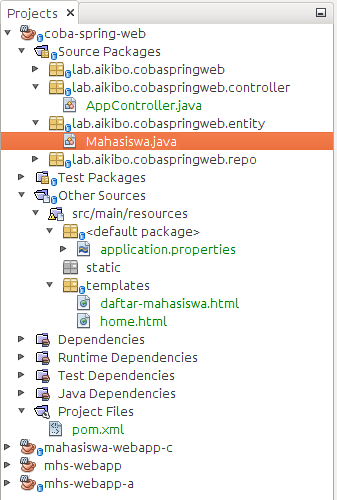
\includegraphics[width=0.5\textwidth]{./resources/012-lokasi-mahasiswa-java}
		\caption{Lokasi \textit{File} \texttt{Mahasiswa.java}}
		\label{fig:lokasi-mahasiswa-java}
	\end{figure}
	
	Isi kode dari \textit{file} \texttt{Mahasiswa.java} ini adalah sebagai berikut :
	
	\begin{lstlisting}
package lab.aikibo.cobaspringweb.entity;

import javax.persistence.Entity;
import javax.persistence.Id;
import lombok.Getter;
import lombok.Setter;

/**
 *
 * @author tamami <tamami.oka@gmail.com>
 */
@Entity
public class Mahasiswa {    
    @Id
    @Getter @Setter
    private String nim;
    
    @Getter @Setter
    private String nama;
    
    @Getter @Setter
    private String jurusan;    
}
	\end{lstlisting}
	
	Kode dari kelas \texttt{Mahasiswa} ini tampak biasa saja, ada tambahan anotasi \texttt{Entity} sebagai penanda bahwa ini adalah kelas entitas, ada anotasi \texttt{Id} yang melekat pada properti \texttt{nim} yang tujuannya adalah memberikan tanda bahwa \textit{primary key} di tabel basis data akan disimpan disini, kemudian ada beberapa anotasi \texttt{Getter} dan \texttt{Setter} yang diambilkan dari pustaka \texttt{lombok} agar kode program yang kita buat lebih bersih dan lebih mudah untuk dibaca.
	
	\item Sampai dengan langkah ini sebetulnya sudah selesai, tinggal dilakukan pengujian pada \textit{browser} dengan terlebih dahulu melakukan \textit{running} pada \textit{project} ini. 
	
	Nantinya di \textit{browser} harus melakukan akses ke \url{localhost:8080/daftar-mahasiswa}, sehingga akan muncul tampilan aplikasi web seperti pada gambar \ref{fig:output-daftar-mahasiswa} berikut :
	
	\begin{figure}[H]
		\centering
		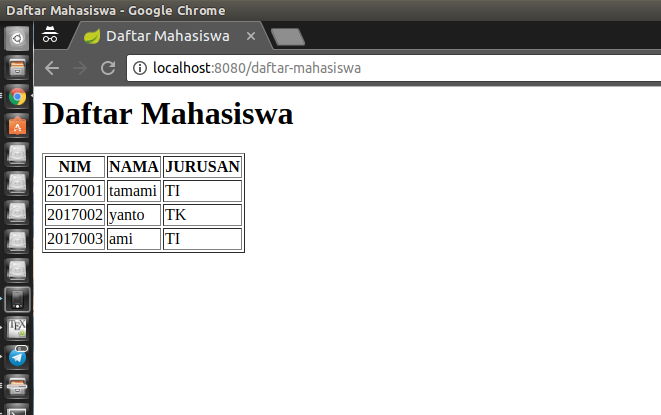
\includegraphics[width=0.8\textwidth]{./resources/013-output-daftar-mahasiswa}
		\caption{Hasil Keluaran Daftar Mahasiswa}
		\label{fig:output-daftar-mahasiswa}
	\end{figure}	
\end{enumerate}

	Sampai sini usaha kita untuk menampilkan data dari tabel ke aplikasi web telah berhasil.

\section{Penambahan Data}

Sekarang waktunya kita berikan fasilitas untuk menambahkan data pada aplikasi web yang kita bangun. Langkah-langkah yang diperlukan adalah sebagai berikut :

\begin{enumerate}
	\item Membuat sebuah halaman \texttt{html} untuk perekaman data dan simpan pada bagian \texttt{Other Sources} pada \textit{folder} \texttt{templates} seperti ditunjukkan oleh gambar \ref{fig:letak-tambah-data} berikut ini :
	
	\begin{figure}[H]
		\centering
		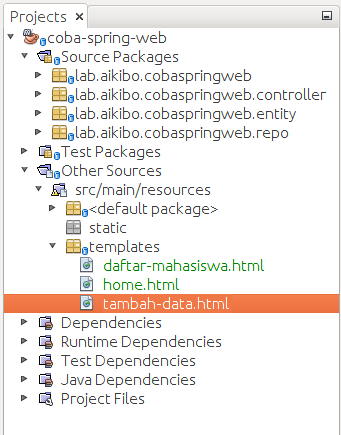
\includegraphics[width=0.5\textwidth]{./resources/014-lokasi-tambah-data}
		\caption{Lokasi \textit{File} \texttt{tambah-data.html}}
		\label{fig:letak-tambah-data}
	\end{figure}
	
	Isi dari \textit{file} ini adalah sebagai berikut :
	
	\begin{lstlisting}
<html xmlns:th="http://www.thymeleaf.org">
<head>
	<title>Formulir Entry Data</title>
</head>

<body>
	<h1>Tambah Data</h1>

	<form th:action="@{/tambah-data}" th:object="${mhs}" method="post">
		<table>
			<tr>
				<td>NIM</td>
				<td><input type="text" th:field="*{nim}" /> </td>
			</tr>
			<tr>
				<td>NAMA</td>
				<td><input type="text" th:field="*{nama}" /></td>
			</tr>
			<tr>
				<td>JURUSAN</td>
				<td><input type="text" th:field="*{jurusan}" /></td>
			</tr>
		</table>
		<button type="submit">Simpan</button>
	</form>
</body>
</html>
	\end{lstlisting}	
	
	Pada baris ke-9 di bagian \texttt{th:action} adalah \textit{url} tujuan dikirimkannya data yang terdapat pada formulir ini, kemudian \texttt{th:object} adalah nama variabel atau identitas objek yang akan dikirim ke \textit{back-end}, sedangkan pada bagian \texttt{method} adalah cara atau metode yang digunakan untuk mengirimkan informasi ke \textit{back-end}. 
	
	Data-data yang dikirim akan disiapkan dalam variabel-variabel atau parameter-parameter pada bagian \texttt{th:field}.
	
	\item Langkah selanjutnya adalah menambahkan sebuah tombol pada \textit{file} \texttt{daftar-mahasiswa.html} dimana skenarionya, pada saat tombol ini diklik, nantinya akan diarahkan ke halaman / formulir \texttt{tambah-data.html}, kemudian \textit{user} / pengguna diberikan kesempatan untuk memasukkan data-data yang diperlukan, kemudian, apabila \textit{user} / pengguna melakukan simpan data, halaman akan dikembalikan ke \texttt{daftar-mahasiswa.html} dengan data baru ikut tampil dalam daftar.
	
	Berikut adalah penambahan isi kode dari file \texttt{daftar-mahasiswa.html} :
	
	\begin{lstlisting}
<html xmlns:th="http://www.thymeleaf.org">
    <head>
        <title>Daftar Mahasiswa</title>
        <meta charset="UTF-8" />
        <meta name="viewport" 
              content="width=device-width, initial-scale=1.0"/>
    </head>
    <body>
        <h1>Daftar Mahasiswa</h1>
        
        <table border="1">
            <thead>
                <tr>
                    <th>NIM</th>
                    <th>NAMA</th>
                    <th>JURUSAN</th>
                </tr>
            </thead>
            <tbody>
                <tr th:each="mhs : ${daftarMahasiswa}">
                    <td th:text="${mhs.nim}"></td>
                    <td th:text="${mhs.nama}"></td>
                    <td th:text="${mhs.jurusan}"></td>
                </tr>
            </tbody>
            (*\textbf{\texttt{<tfoot> }}*)
                (*\textbf{\texttt{<tr> }}*)
                    (*\textbf{\texttt{<td><a href="/tambah-data.html">}}*)
                        (*\textbf{\texttt{Tambah}}*)
                    (*\textbf{\texttt{</a></td>}}*)
                (*\textbf{\texttt{</tr> }}*)
            (*\textbf{\texttt{</tfoot> }}*)
        </table>
    </body>
</html>
	\end{lstlisting}
	
	\item Selanjutnya agar \textit{file} tersebut dapat muncul di \textit{browser}, maka kita perlu menambahkan \textit{controler} sebuah \textit{mapping} yang mengarahkan ke \texttt{tambah-data.html}, berikut adalah hasil perubahan kode \texttt{AppController} :
	
	\begin{lstlisting}
package lab.aikibo.cobaspringweb.controller;

import lab.aikibo.cobaspringweb.entity.Mahasiswa;
import lab.aikibo.cobaspringweb.repo.MahasiswaRepo;
import org.springframework.beans.factory.annotation.Autowired;
import org.springframework.stereotype.Controller;
import org.springframework.ui.Model;
import org.springframework.validation.BindingResult;
import org.springframework.web.bind.annotation.ModelAttribute;
import org.springframework.web.bind.annotation.RequestMapping;
import org.springframework.web.bind.annotation.RequestMethod;

/**
 *
 * @author tamami <tamami.oka@gmail.com>
 */
@Controller
public class AppController {
    
    @Autowired
    private MahasiswaRepo mhsRepo;
    
    @RequestMapping("/home")
    public void index() {}
    
    @RequestMapping("/daftar-mahasiswa") 
    public void getDaftarMahasiswa(Model model) {
        model.addAttribute("daftarMahasiswa", mhsRepo.findAll());
    }
    

    (*\textbf{\texttt{@RequestMapping(value = "/tambah-data",}}*)
        (*\textbf{\texttt{method = RequestMethod.GET) }}*)
    (*\textbf{\texttt{public void getTambahData( }}*)
            (*\textbf{\texttt{@ModelAttribute("mhs")Mahasiswa mhs, }}*)
            (*\textbf{\texttt{BindingResult binding) \{ }}*)
    (*\textbf{\texttt{\} }}*)
    
}	
	\end{lstlisting}
	
	Perhatikan pada baris ke-32 bahwa \textit{mapping} yang disiapkan adalah untuk \textit{url} \texttt{/tambah-data}, dengan \texttt{RequestMethod.GET}.
	
	\item Melakukan pemeriksaan tampilan dengan menjalankan dan mengaksesnya melalui \textit{browser}. Nantinya akan muncul jendela seperti gambar \ref{fig:form-add-data} berikut :
	
	\begin{figure}[H]
		\centering
		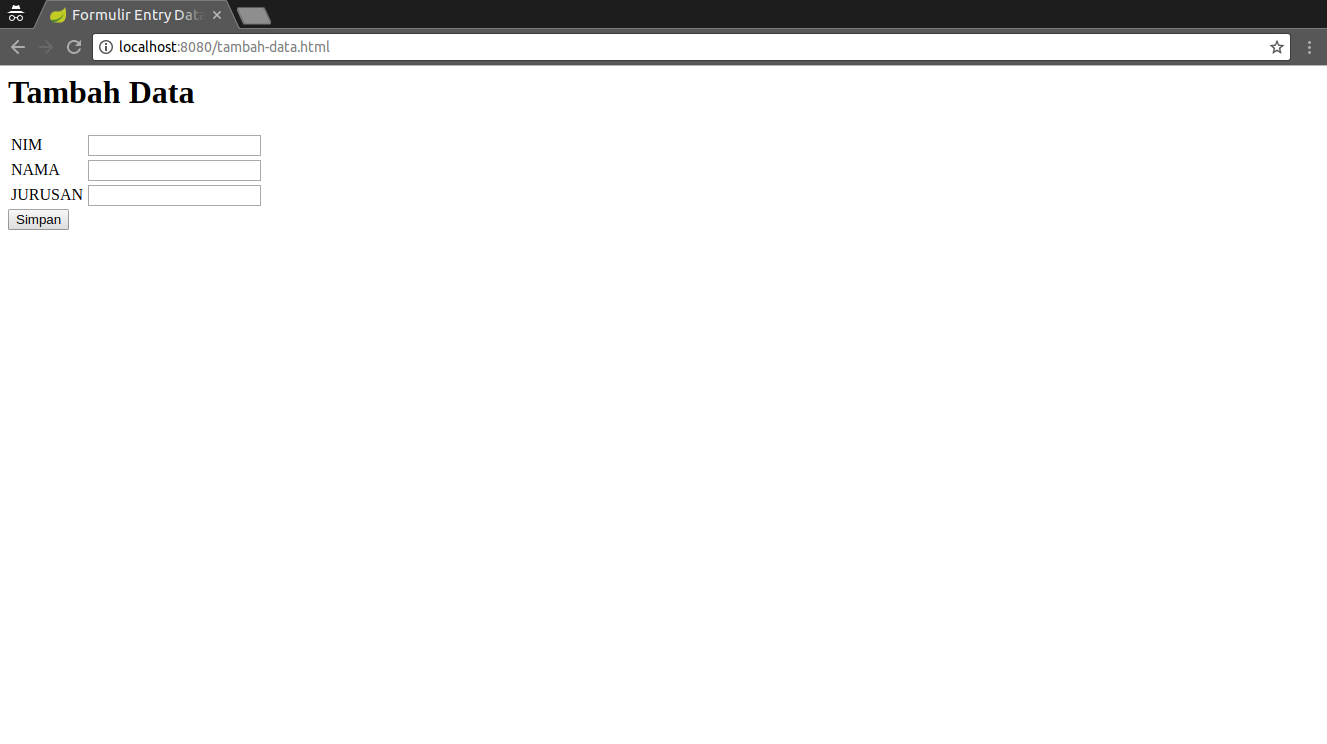
\includegraphics[width=1\textwidth]{./resources/015-form-add-data}
		\caption{Tampilan Formulir Tambah Data}
		\label{fig:form-add-data}
	\end{figure}
	
	Formulir tersebut hanya berupa tampilan yang belum memiliki respon apapun.

	\item Agar tombol \texttt{Simpan} dapat berfungsi, kita harus siapkan sebuah \textit{mapping} dengan \textit{url} \texttt{/tambah-data} dengan metode \texttt{RequestMethod.POST}. Berikut adalah  kode tambahan untuk \texttt{AppController} yang telah kita buat :
	
	\begin{lstlisting}
package lab.aikibo.cobaspringweb.controller;

import lab.aikibo.cobaspringweb.entity.Mahasiswa;
import lab.aikibo.cobaspringweb.repo.MahasiswaRepo;
import org.springframework.beans.factory.annotation.Autowired;
import org.springframework.stereotype.Controller;
import org.springframework.ui.Model;
import org.springframework.validation.BindingResult;
import org.springframework.web.bind.annotation.ModelAttribute;
import org.springframework.web.bind.annotation.RequestMapping;
import org.springframework.web.bind.annotation.RequestMethod;

/**
 *
 * @author tamami <tamami.oka@gmail.com>
 */
@Controller
public class AppController {
    
    @Autowired
    private MahasiswaRepo mhsRepo;
    
    @RequestMapping("/home")
    public void index() {}
    
    @RequestMapping("/daftar-mahasiswa") 
    public void getDaftarMahasiswa(Model model) {
        model.addAttribute("daftarMahasiswa", mhsRepo.findAll());
    }
    
    @RequestMapping(value = "/tambah-data", method = RequestMethod.GET)
    public void getTambahData(@ModelAttribute("mhs")Mahasiswa mhs, 
            BindingResult binding) {
    }
    
    (*\textbf{\texttt{@RequestMapping(value = "/tambah-data",}}*)
        (*\textbf{\texttt{method = RequestMethod.POST)}} *)
    (*\textbf{\texttt{public String saveTambahData(}}*)
            (*\textbf{\texttt{@ModelAttribute("mhs")Mahasiswa mhs,}}*)
            (*\textbf{\texttt{BindingResult binding) \{ }}*)
        (*\textbf{\texttt{System.out.println(mhs.getNim());}}*)
        (*\textbf{\texttt{mhsRepo.save(mhs);}}*)
        (*\textbf{\texttt{return "redirect:/daftar-mahasiswa";}}*)
    (*\textbf{\texttt{\} }}*)
    
}
	\end{lstlisting}
	
	Pada baris ke-37 kita melihat bahwa \textit{method} ini akan dieksekusi saat ada permintaan \texttt{post} pada \textit{url} \texttt{/tambah-data}, pada baris ke-41 hanya untuk memastikan bahwa data yang dikirim dari \textit{front-end} atau \textit{user-interface} telah sampai ke \textit{back-end}.
	
	Perintah pada baris ke-42 adalah perintah inti, karena pada saat \textit{request} \texttt{post} terjadi pada \textit{url} \texttt{/tambah-data}, maka data yang terkirim harus tersimpan dalam basis data, untuk hal ini, kita menggunakan Spring Data JPA Repository untuk melakukan simpan data.
	
	Setelah semua selesai dikerjakan, maka kembalikan tampilan yang ada menjadi daftar mahasiswa kembali dengan perintah seperti pada baris ke-43.
	
	Setelah diuji, seharusnya data yang baru telah tersimpan dalam basis data dan data baru secara otomatis akan muncul pada daftar mahasiswa.
	
\end{enumerate}

Sampai sini fasilitas untuk menambahkan data ke dalam tabel di basis data selesai.

\section{Pengubahan Data}

Kali ini kita akan memberikan sebuah fasilitas agar \textit{user} dapat mengubah data yang telah tersimpan dalam basis data. Langkahnya adalah sebagai berikut :

\begin{enumerate}
	\item Pada \textit{file} \texttt{daftar-mahasiswa\.html}, kita berikan pilihan atau tombol \texttt{ubah} untuk mengubah data yang ada, berikut perubahan kode yang terjadi pada \textit{file} tersebut :
	
	\begin{lstlisting}
<html xmlns:th="http://www.thymeleaf.org">
    <head>
        <title>Daftar Mahasiswa</title>
        <meta charset="UTF-8" />
        <meta name="viewport" 
              content="width=device-width, initial-scale=1.0"/>
    </head>
    <body>
        <h1>Daftar Mahasiswa</h1>
        
        <table border="1">
            <thead>
                <tr>
                    <th>NIM</th>
                    <th>NAMA</th>
                    <th>JURUSAN</th>
                </tr>
            </thead>
            <tbody>
                <tr th:each="mhs : ${daftarMahasiswa}">
                    <td th:text="${mhs.nim}"></td>
                    <td th:text="${mhs.nama}"></td>
                    <td th:text="${mhs.jurusan}"></td>
                    (*\textbf{\texttt{<td> }}*)
                      (*\textbf{\texttt{<a href="@\{/edit(nim=\$\{mhs.nim\})\}"> }}*)
                        (*\textbf{\texttt{Ubah }}*)
                      (*\textbf{\texttt{ </a> }}*) 
                    (*\textbf{\texttt{</td> }}*)
                </tr>
            </tbody>
            <tfoot>
                <tr>
                    <td><a href="/tambah-data.html">Tambah</a></td>
                </tr>
            </tfoot>
        </table>
    </body>
</html>
	\end{lstlisting}

Pada baris ke-25 kita memberikan identitas untuk tiap baris yang muncul di tabel, sehingga tombol \texttt{Ubah} manapun yang diklik akan memberikan informasi data mahasiswa dengan NIM mana yang akan diubah.

Nantinya \textit{url} yang akan muncul saat tombol \texttt{Ubah} diklik akan berbentuk seperti ini \texttt{/edit?nim=\{nim\}}

	\item Langkah berikutnya adalah menyiapkan \textit{controller} untuk alamat yang diinginkan dari \textit{edit} data tersebut, berikut adalah perubahan kode yang terjadi di kelas \texttt{AppController} :
	
	\begin{lstlisting}
package lab.aikibo.cobaspringweb.controller;

import lab.aikibo.cobaspringweb.entity.Mahasiswa;
import lab.aikibo.cobaspringweb.repo.MahasiswaRepo;
import org.springframework.beans.factory.annotation.Autowired;
import org.springframework.stereotype.Controller;
import org.springframework.ui.Model;
import org.springframework.validation.BindingResult;
import org.springframework.web.bind.annotation.ModelAttribute;
import org.springframework.web.bind.annotation.RequestMapping;
import org.springframework.web.bind.annotation.RequestMethod;
import org.springframework.web.bind.annotation.RequestParam;


/**
 *
 * @author tamami <tamami.oka@gmail.com>
 */
@Controller
public class AppController {
    
    @Autowired
    private MahasiswaRepo mhsRepo;
    
    @RequestMapping("/home")
    public void index() {}
    
    @RequestMapping("/daftar-mahasiswa") 
    public void getDaftarMahasiswa(Model model) {
        model.addAttribute("daftarMahasiswa", mhsRepo.findAll());
    }
    
    @RequestMapping(value = "/tambah-data", method = RequestMethod.GET)
    public void getTambahData(@ModelAttribute("mhs")Mahasiswa mhs, 
            BindingResult binding) {
    }
    
    @RequestMapping(value = "/tambah-data", method = RequestMethod.POST) 
    public String saveTambahData(@ModelAttribute("mhs")Mahasiswa mhs,
            BindingResult binding) {
        System.out.println(mhs.getNim());
        mhsRepo.save(mhs);
        return "redirect:/daftar-mahasiswa";
    }

    (*\textbf{\texttt{@RequestMapping(value = "/edit", method = RequestMethod.GET) }}*)
    (*\textbf{\texttt{public void getEditData(@RequestParam(name = "nim", required = false) String nim, }}*)
        (*\textbf{\texttt{@ModelAttribute("mhs") Mahasiswa mahasiswa, BindingResult binding) \{ }}*)
      (*\textbf{\texttt{Mahasiswa mhs = mhsRepo.findByNim(nim); }}*)
      (*\textbf{\texttt{mahasiswa.setNim(mhs.getNim()); }}*)
      (*\textbf{\texttt{mahasiswa.setNama(mhs.getNama()); }}*)
      (*\textbf{\texttt{mahasiswa.setJurusan(mhs.getJurusan()); }}*)
    (*\textbf{\texttt{\} }}*)
}
	\end{lstlisting}

	\textit{Method} tersebut akan merespon dengan tampilnya halaman \texttt{edit.html}, parameter \texttt{nim} yang dikirimkan oleh \textit{client} akan dicarikan datanya seperti pada baris ke-49, kemudian hasil pencarian akan disimpan dalam variabel \texttt{mhs} yang dikembalikan ke halaman \texttt{edit.html}.
	
	\item Membuat halaman \texttt{edit.html} untuk memberikan kesempatan \textit{user} melakukan perubahan data, berikut isi kode dari \texttt{edit.html} :
	
	\begin{lstlisting}
<html xmlns:th="http://www.thymeleaf.org">
<head>
	<title>Formulir Ubah Data</title>
</head>

<body>
	<h1>Ubah Data</h1>

	<form th:action="@{/edit}" th:object="${mhs}" method="post">
		<table>
			<tr>
				<td>NIM</td>
				<td><input type="text" th:field="*{nim}" disabled="true" /> </td>
				<td><input type="hidden" th:field="*{nim}" /></td>
			</tr>
			<tr>
				<td>NAMA</td>
				<td><input type="text" th:field="*{nama}" /></td>
			</tr>
			<tr>
				<td>JURUSAN</td>
				<td><input type="text" th:field="*{jurusan}" /></td>
			</tr>
		</table>
		<button type="submit">Simpan</button>
	</form>
</body>
</html>
	\end{lstlisting}
	
	Kode ini sama seperti kode untuk \textit{entry} data, hanya saja pada saat data dikirimkan akan menuju ke \textit{url} \texttt{/edit} dengan metode \textit{post}.
	
	\item Melakukan perubahan pada kelas \texttt{AppController} agar dapat menangani metode \textit{post} pada \textit{url} \texttt{/edit}, berikut perubahan kode yang terjadi pada kelas \texttt{AppController} :
	
	\begin{lstlisting}
package lab.aikibo.cobaspringweb.controller;

import lab.aikibo.cobaspringweb.entity.Mahasiswa;
import lab.aikibo.cobaspringweb.repo.MahasiswaRepo;
import org.springframework.beans.factory.annotation.Autowired;
import org.springframework.stereotype.Controller;
import org.springframework.ui.Model;
import org.springframework.validation.BindingResult;
import org.springframework.web.bind.annotation.ModelAttribute;
import org.springframework.web.bind.annotation.RequestMapping;
import org.springframework.web.bind.annotation.RequestMethod;
import org.springframework.web.bind.annotation.RequestParam;


/**
 *
 * @author tamami <tamami.oka@gmail.com>
 */
@Controller
public class AppController {
    
    @Autowired
    private MahasiswaRepo mhsRepo;
    
    @RequestMapping("/home")
    public void index() {}
    
    @RequestMapping("/daftar-mahasiswa") 
    public void getDaftarMahasiswa(Model model) {
        model.addAttribute("daftarMahasiswa", mhsRepo.findAll());
    }
    
    @RequestMapping(value = "/tambah-data", method = RequestMethod.GET)
    public void getTambahData(@ModelAttribute("mhs")Mahasiswa mhs, 
            BindingResult binding) {
    }
    
    @RequestMapping(value = "/tambah-data", method = RequestMethod.POST) 
    public String saveTambahData(@ModelAttribute("mhs")Mahasiswa mhs,
            BindingResult binding) {
        System.out.println(mhs.getNim());
        mhsRepo.save(mhs);
        return "redirect:/daftar-mahasiswa";
    }

    @RequestMapping(value = "/edit", method = RequestMethod.GET)
    public void getEditData(@RequestParam(name = "nim", required = false) String nim, 
    	@ModelAttribute("mhs") Mahasiswa mahasiswa, BindingResult binding) {
    	Mahasiswa mhs = mhsRepo.findByNim(nim);
    	mahasiswa.setNim(mhs.getNim());
    	mahasiswa.setNama(mhs.getNama());
    	mahasiswa.setJurusan(mhs.getJurusan());
    }

    (*\textbf{\texttt{@RequestMapping(value = "/edit", }}*) 
        (*\textbf{\texttt{method = RequestMethod.POST) }}*)
    (*\textbf{\texttt{public String saveEditData( }}*)
        (*\textbf{\texttt{@ModelAttribute("mhs") Mahasiswa mhs, }}*)
        (*\textbf{\texttt{BindingResult binding) \{ }}*)
      (*\textbf{\texttt{mhsRepo.save(mhs); }}*)
      (*\textbf{\texttt{return "redirect:/daftar-mahasiswa"; }}*)
    (*\textbf{\texttt{\} }}*)
    
}
	\end{lstlisting}
	
	Pada kode tersebut, sama seperti metode \textit{get} di atasnya, memiliki \texttt{ModelAttribute} dan \texttt{BindingResult}, jadi perintahnya apabila metode ini dieksekusi, maka langsung saja simpan perubahannya pada basis data seperti perintah pada baris ke-60, dan kembalikan tampilannya ke \texttt{/daftar-mahasiswa} agar perubahan langsung dapat ditampilkan.
	
	Sampai sini operasi perubahan data pada basis data selesai.

\end{enumerate}

\section{Penghapusan Data}

Pada bagian ini akan kita bahas bagaimana cara menghapus sebuah data di basis data melalui aplikasi web yang telah kita bangun. Secara konsep akan mirip seperti saat kita memberikan fasilitas perubahan data, ada identitas unik untuk tiap baris yang kita kirimkan ke \textit{backend service}, kebetulan yang menjadi identitas unik ini adalah NIM dari tiap mahasiswa, sehingga NIM ini akan kita lewatkan atau kita jadikan salah satu parameter \textit{request} yang dikirim ke \textit{backend service}.

Langkah-langkahnya adalah sebagai berikut :

\begin{enumerate}
	\item Pertama kita ubah terlebih dahulu \textit{file} \texttt{daftar-mahasiswa.html} sehingga kodenya menjadi terlihat seperti ini :
	
	\begin{lstlisting}
<html xmlns:th="http://www.thymeleaf.org">
    <head>
        <title>Daftar Mahasiswa</title>
        <meta charset="UTF-8" />
        <meta name="viewport" 
              content="width=device-width, initial-scale=1.0"/>
    </head>
    <body>
        <h1>Daftar Mahasiswa</h1>
        
        <table border="1">
            <thead>
                <tr>
                    <th>NIM</th>
                    <th>NAMA</th>
                    <th>JURUSAN</th>
                </tr>
            </thead>
            <tbody>
                <tr th:each="mhs : ${daftarMahasiswa}">
                    <td th:text="${mhs.nim}"></td>
                    <td th:text="${mhs.nama}"></td>
                    <td th:text="${mhs.jurusan}"></td>
                    <td><a th:href="@{/edit(nim=${mhs.nim})}">Ubah</a></td>     
                    (*\textbf{\texttt{<td> }}*)
                      (*\textbf{\texttt{<a th:href="@\{/delete(nim=\$\{mhs.nim\})\}"> }}*)
                        (*\textbf{\texttt{Hapus }}*)
                      (*\textbf{\texttt{</a> }}*)
                    (*\textbf{\texttt{</td> }}*)
                </tr>
            </tbody>
            <tfoot>
                <tr>
                    <td><a href="/tambah-data.html">Tambah</a></td>
                </tr>
            </tfoot>
        </table>
    </body>
</html>
	\end{lstlisting}
	
	\item Karena \textit{url} yang dituju belum didefinisikan di \textit{controller}, maka kita akan mengubah kode kelas \texttt{AppController} yang kita miliki menjadi seperti ini :
	
	\begin{lstlisting}
package lab.aikibo.cobaspringweb.controller;

import lab.aikibo.cobaspringweb.entity.Mahasiswa;
import lab.aikibo.cobaspringweb.repo.MahasiswaRepo;
import org.springframework.beans.factory.annotation.Autowired;
import org.springframework.stereotype.Controller;
import org.springframework.ui.Model;
import org.springframework.validation.BindingResult;
import org.springframework.web.bind.annotation.ModelAttribute;
import org.springframework.web.bind.annotation.RequestMapping;
import org.springframework.web.bind.annotation.RequestMethod;
import org.springframework.web.bind.annotation.RequestParam;


/**
 *
 * @author tamami <tamami.oka@gmail.com>
 */
@Controller
public class AppController {
    
    @Autowired
    private MahasiswaRepo mhsRepo;
    
    @RequestMapping("/home")
    public void index() {}
    
    @RequestMapping("/daftar-mahasiswa") 
    public void getDaftarMahasiswa(Model model) {
        model.addAttribute("daftarMahasiswa", mhsRepo.findAll());
    }
    
    @RequestMapping(value = "/tambah-data", method = RequestMethod.GET)
    public void getTambahData(@ModelAttribute("mhs")Mahasiswa mhs, 
            BindingResult binding) {
    }
    
    @RequestMapping(value = "/tambah-data", method = RequestMethod.POST) 
    public String saveTambahData(@ModelAttribute("mhs")Mahasiswa mhs,
            BindingResult binding) {
        System.out.println(mhs.getNim());
        mhsRepo.save(mhs);
        return "redirect:/daftar-mahasiswa";
    }

    @RequestMapping(value = "/edit", method = RequestMethod.GET)
    public void getEditData(@RequestParam(name = "nim", required = false) String nim, 
    	@ModelAttribute("mhs") Mahasiswa mahasiswa, BindingResult binding) {
    	Mahasiswa mhs = mhsRepo.findByNim(nim);
    	mahasiswa.setNim(mhs.getNim());
    	mahasiswa.setNama(mhs.getNama());
    	mahasiswa.setJurusan(mhs.getJurusan());
    }

    @RequestMapping(value = "/edit", method = RequestMethod.POST)
    public String saveEditData(@ModelAttribute("mhs") Mahasiswa mhs, 
    		BindingResult binding) {
    	mhsRepo.save(mhs);
    	return "redirect:/daftar-mahasiswa";
    }

    (*\textbf{\texttt{@RequestMapping("/delete") }}*)
    (*\textbf{\texttt{public String deleteData( }}*)
        (*\textbf{\texttt{@RequestParam(name = "nim", required = true) String nim) \{ }}*)
      (*\textbf{\texttt{mhsRepo.delete(nim); }}*)
      (*\textbf{\texttt{return "redirect:/daftar-mahasiswa"; }}*)
    (*\textbf{\texttt{\} }}*)
    
}
	\end{lstlisting}
	
	Perintahnya cukup sederhana, dari parameter NIM yang dikirimkan oleh \textit{browser}, kita cukup memanggil \textit{method} \texttt{delete} milik \texttt{JpaRepository} berdasarkan \textit{primary key}, kemudian mengembalikan halaman \textit{browser} ke \textit{url} \texttt{/daftar-mahasiswa}.
\end{enumerate}

Cukup 2 (dua) perubahan tersebut, kita sudah menyelesaikan fasilitas hapus data pada aplikasi perekaman data mahasiswa yang kita bangun.

Sekarang lengkap sudah fasilitas yang ada pada aplikasi web perekaman data mahasiswa, untuk selanjutnya dapat dikembangkan atau diimplementasikan pada soal UTS.